\subsection{Reunión grupal}

  \paragraph{}La gestión de las reuniones grupales para el usuario
  \textit{Asesor} es idéntica a la comentada para el usuario
  \textit{Administrador principal} en la sección \ref{gestionReunion},
  con la diferencia de que solo estarán disponibles los alumnos a los que
  este usuario preste asesoría en el curso académico actual.

  \paragraph{}Además, la forma de convocar alumnos para que participen en dicha
  reunión cambia con respecto a la forma de crear reuniones vista anteriormente.
  De esta forma, es posible convocar a un alumno para que participe en la
  reunión mediante el icono \textit{Participa}, como el que muestra la figura
  \ref{capturaIconoParticipa}.

  \begin{figure}[!ht]
    \begin{center}
      \fbox{
      
\includegraphics[scale=0.6]{4.Funcionamiento_Aplicacion/4.3.Gestion/4.3.3.Asesor/4.3.3.8.ReunionGrupal/iconoParticipa.png}
      }
      \caption{Captura de pantalla del icono \textit{Participa}.}
      \label{capturaIconoParticipa}
    \end{center}
  \end{figure}

  \paragraph{}Si hemos convocado a un alumno a esta reunión por error, se puede
  desconvocar su participación mediante el icono \textit{No participa}, el cual
  se puede ver en la figura \ref{capturaIconoNoParticipa}.

  \begin{figure}[!ht]
    \begin{center}
      \fbox{
      
\includegraphics[scale=0.6]{4.Funcionamiento_Aplicacion/4.3.Gestion/4.3.3.Asesor/4.3.3.8.ReunionGrupal/iconoNoParticipa.png}
      }
      \caption{Captura de pantalla del icono \textit{No participa}.}
      \label{capturaIconoNoParticipa}
    \end{center}
  \end{figure}

  \paragraph{}La figura \ref{capturaReunionGrupal} muestra la pantalla de
  creación de una reunión grupal.

  \begin{figure}[!ht]
    \begin{center}
      \fbox{
      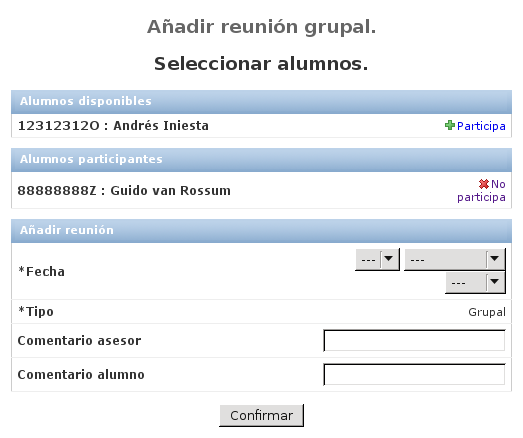
\includegraphics[scale=0.6]{4.Funcionamiento_Aplicacion/4.3.Gestion/4.3.3.Asesor/4.3.3.8.ReunionGrupal/add_reunion_grupal.png}
      }
      \caption{Captura de pantalla de la creación de \textit{Reunión grupal}.}
      \label{capturaReunionGrupal}
    \end{center}
  \end{figure}

  \paragraph{}Desde este listado, el usuario asesor podrá añadir preguntas,
  bien oficiales o bien de reunión, a una reunión grupal, además de ver las
  ya existentes. La figura \ref{capturaPantallaReunionGrupal} muestra esta
  ventana.

  \begin{figure}[!ht]
    \begin{center}
      \fbox{
      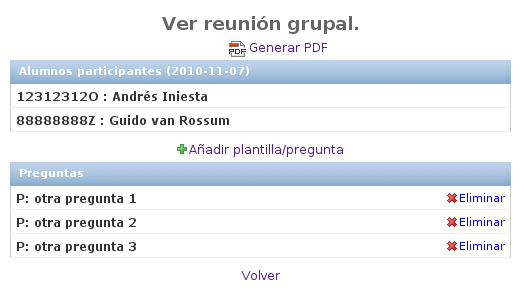
\includegraphics[scale=0.55]{4.Funcionamiento_Aplicacion/4.3.Gestion/4.3.3.Asesor/4.3.3.8.ReunionGrupal/lista_reunion.png}
      }
      \caption{Captura de pantalla del listado de una reunión grupal para el usuario \textit{Asesor}.}
      \label{capturaPantallaReunionGrupal}
    \end{center}
  \end{figure}

  \paragraph{}Al pulsar en el enlace \textit{Añadir plantilla/pregunta},
  aparecerá una ventana con las plantillas y preguntas disponibles para este
  usuario. Esta ventana es la mostrada en la figura
  \ref{capturaPantallaAddPlantillaReunionGru}.

  \begin{figure}[!ht]
    \begin{center}
      \fbox{
      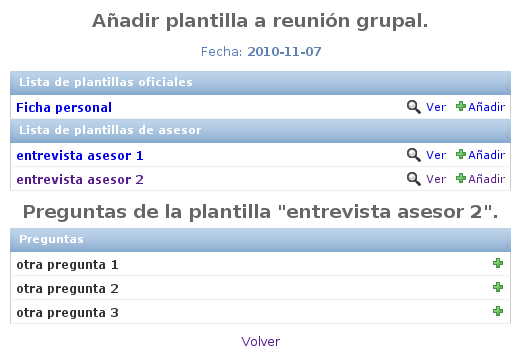
\includegraphics[scale=0.55]{4.Funcionamiento_Aplicacion/4.3.Gestion/4.3.3.Asesor/4.3.3.8.ReunionGrupal/add_plantilla.png}
      }
      \caption{Captura de pantalla del listado de plantillas y preguntas grupales para el usuario \textit{Asesor}.}
      \label{capturaPantallaAddPlantillaReunionGru}
    \end{center}
  \end{figure}
